UML je jazyk umožňující \textbf{specifikaci} (struktura a model), \textbf{vizualizaci} (grafy), \textbf{konstrukci} (vygenerování kódu, např class diagram) a \textbf{dokumentaci artefaktů} softwarového systému. V průběhu let se UML stal \textbf{standardizovaným jazykem }určeným pro vytvoření výkresové dokumentace (softwarového) systému v \textbf{různých fázích vývoje}. K vytváření jednotlivých modelů systému jazyk UML poskytuje celou řadu diagramů umožňujících \textbf{postihnout různé aspekty systému}. Jedná se celkem o čtyři základní náhledy a k nim přiřazené diagramy: 

\begin{enumerate}
\item \textbf{Funkční náhled}
\begin{enumerate}
\item \textbf{Diagram případů užití} -- popisuje vztahy mezi aktéry a jednotlivými případy použití. Poskytuje funčkní náhled na systém (kdo se systémem pracuje a jak). Uplatňuje se pro realizaci \textbf{DFD} (Data flow diagram) ve fázi \textbf{specifikace požadavků} (VIS).
\end{enumerate}
\item \textbf{Logický náhled}
\begin{enumerate}
\item \textbf{Diagram tříd} -- specifikuje množinu tříd, rozhraní a jejich vzájemné vztahy. Tyto diagramy slouží k vyjádření statického pohledu na systém.
\begin{figure}[H]
	\centering
	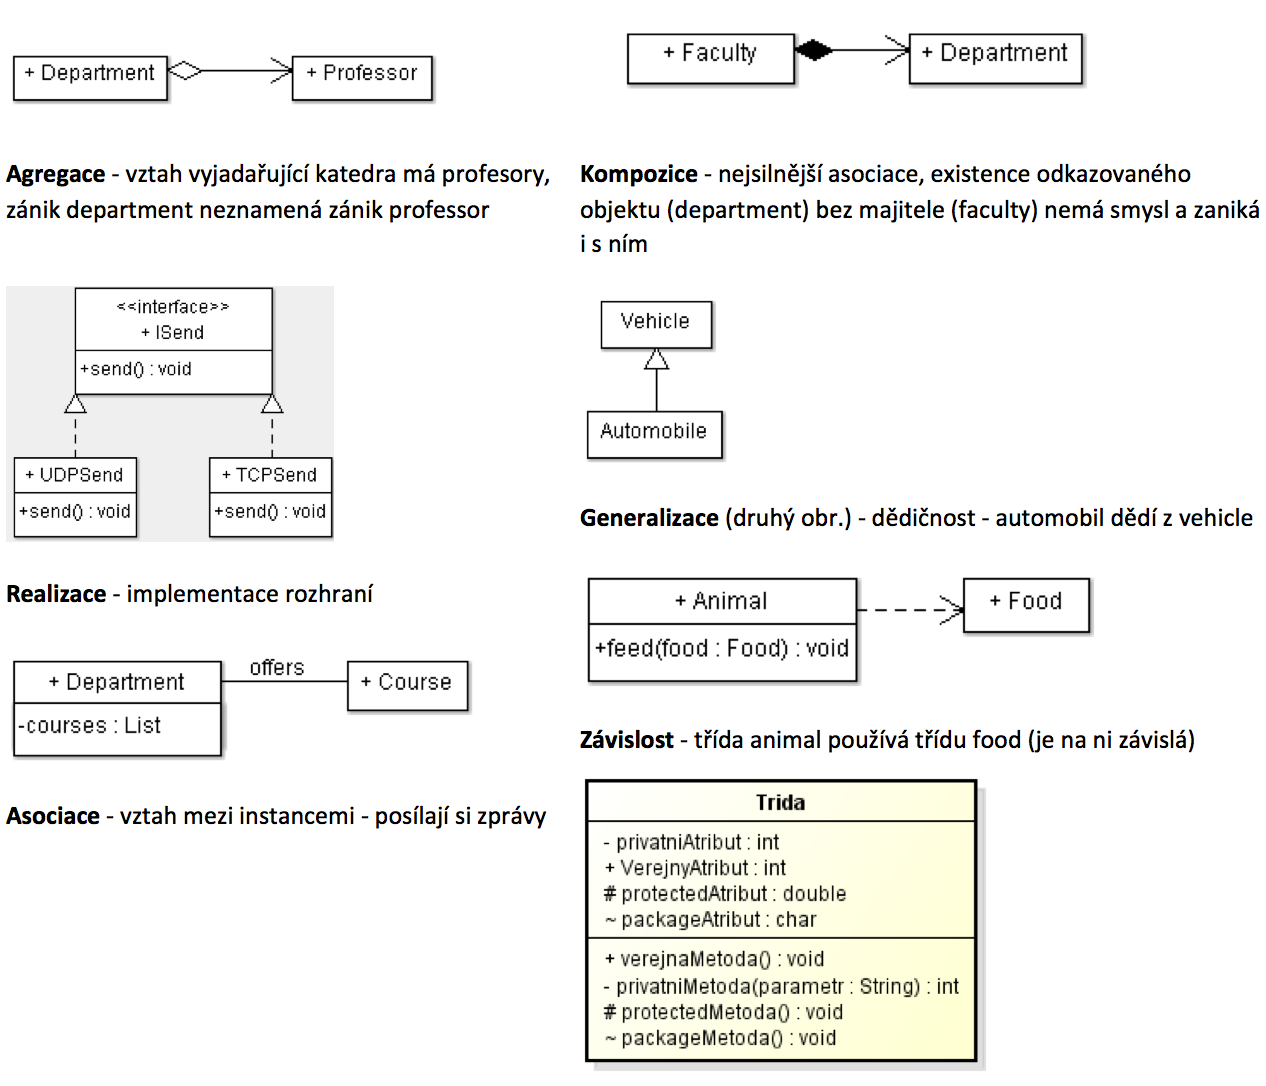
\includegraphics[width=.9\textwidth]{assets/class.png}
\end{figure}
\item \textbf{Objektový diagram} -- zobrazuje \textbf{instance tříd} (objekty), někdy nazýván jako instanční diagram.
Je \textbf{snímkem objektů} a jejich vztahů v systému \textbf{v určitém časovém okamžiku}, který chceme z nějakého důvodu zdůraznit. Využívá se v datové analýze pro ERD.
\begin{figure}[H]
	\centering
	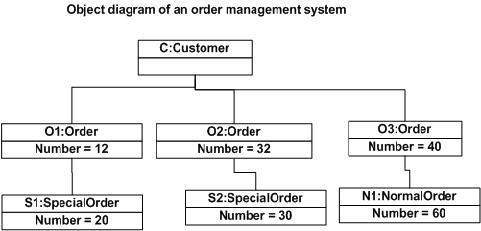
\includegraphics[width=.5\textwidth]{assets/obj_diag.jpg}
\end{figure}
\end{enumerate}

\item \textbf{Dynamický náhled popisující chování}
\begin{enumerate}
\item \textbf{Stavový diagram} -- dokumentuje \textbf{životní cyklus} objektu dané třídy z hlediska jeho \textbf{stavů}, \textbf{přechodů} mezi těmito stavy a \textbf{událostmi}, které tyto přechody uskutečňují. 
\begin{figure}[H]
	\centering
	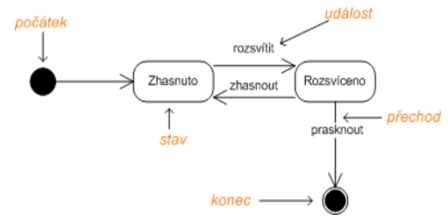
\includegraphics[width=.5\textwidth]{assets/stav_diag.png}
\end{figure}
\item \textbf{Diagram aktivit} --  popisuje podnikový proces pomocí jeho stavů reprezentovaných vykonáváním aktivit a pomocí přechodů mezi těmito stavy způsobených ukončením těchto aktivit. Účelem diagramu aktivit je blíže popsat tok činností daný vnitřním mechanismem jejich provádění. 
\item \textbf{Sekvenční diagramy} -- popisuje interkace mezi objekty z hlediska jejich \textbf{časového uspořádaní}.
\item \textbf{Diagramy spolupráce} -- je obdobně jako předchozí sekvenční diagram zaměřen na interkace, ale z pohledu strukturální organizace objektů. Jinými slovy není primárním aspektem časová posloupnost posílaných zpráv, ale \textbf{topologie rozmístění objektů}.

Časová posloupnost zaslání zpráv je vyjádřena jejich \textbf{pořadovým číslem}. Návratová hodnota je vyjádřena \textbf{operátorem přířazení} \textbf{$:=$}. Opakované zaslání zprávy je dáno symbolem \textbf{*} a v hranatých závorkách uvedením podmínky opakování cyklu. Navíc tento diagram zavádí i následující \textbf{typy viditelnosti} vzájemně spojených objektů: 
\begin{enumerate}
\item \texttt{<<local>>} -- vyjadřuje situaci, kdy objekt je vytvořen v těle operace a po jejím vykonání je zrušen, 
\item \texttt{<<global>>} -- specifikuje globálně viditelný objekt,
\item \texttt{<<parameter>>} -- vyjadřuje fakt, že objekt je předán druhému jako argument na něj zaslané zprávy,
\item \texttt{<<association>>} -- specifikuje trvalou vazbu mezi objekty (někdy se také hovoří o tzv. známostním spojení).
\end{enumerate}

\begin{figure}[H]
	\centering
	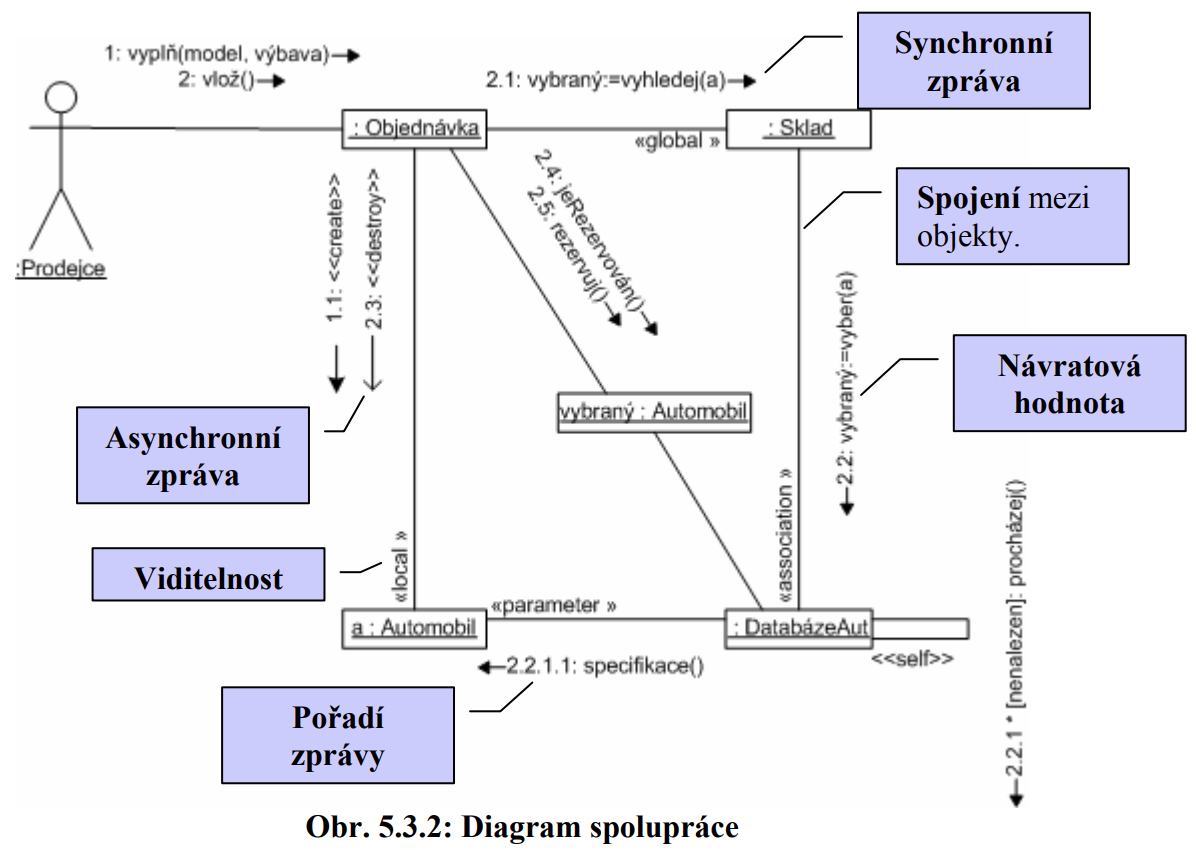
\includegraphics[width=.8\textwidth]{assets/diag_spoluprace.png}
\end{figure}
\end{enumerate}
\item \textbf{Implementační náhled}
\begin{enumerate}
\item \textbf{Diagram komponent} -- ilustruje organizaci a \textbf{závislosti mezi softwarovými komponentami}. Zdrojové komponenty tvoří soubory vytvořené použitým programovacím jazykem. Diagram spustitelných komponent specifikuje všechny komponenty vytvořené námi i ty, které nám dává k dispozici implementační prostředí.
\item \textbf{Diagram nasazení} -- upřesňuje nejen ve smyslu konfigurace technických prostředků, ale především z hlediska rozmístění implementovaných softwarových komponent na těchto prostředcích.
\end{enumerate}
\end{enumerate}


\subsection{Diagramy a jejich použití v rámci fází vývoje}
\begin{itemize}
\item \textbf{Specifikace požadavků}: Diagram případů užití, Sekvenční diagramy, Diagram aktivit.
\item \textbf{Návrh}: Diagram tříd, Objektový diagram, Stavový diagram, Sekvenční diagramy.
\item \textbf{Implementace}: Diagramy spolupráce, Diagram komponent, Diagram nasazení.
\end{itemize}
